%%%%%%%%%%%%%%%%%%%%%%%%%%%%%%%%%%%%%%%%%
% Masters/Doctoral Thesis 
% LaTeX Template
% Version 1.42 (19/1/14)
%
% This template has been downloaded from:
% http://www.latextemplates.com
%
% Original authors:
% Steven Gunn 
% http://users.ecs.soton.ac.uk/srg/softwaretools/document/templates/
% and
% Sunil Patel
% http://www.sunilpatel.co.uk/thesis-template/
%
% License:
% CC BY-NC-SA 3.0 (http://creativecommons.org/licenses/by-nc-sa/3.0/)
%
% Note:
% Make sure to edit document variables in the Thesis.cls file
%
%%%%%%%%%%%%%%%%%%%%%%%%%%%%%%%%%%%%%%%%%

%----------------------------------------------------------------------------------------
%	PACKAGES AND OTHER DOCUMENT CONFIGURATIONS
%----------------------------------------------------------------------------------------

\documentclass[11pt, a4paper, oneside]{Thesis} % Paper size, default font size and one-sided paper

\graphicspath{{Pictures/}} % Specifies the directory where pictures are stored

\usepackage[square, numbers, comma, sort&compress]{natbib} % Use the natbib reference package - read up on this to edit the reference style; if you want text (e.g. Smith et al., 2012) for the in-text references (instead of numbers), remove 'numbers' 
\usepackage{listings}
\hypersetup{urlcolor=blue, colorlinks=true} % Colors hyperlinks in blue - change to black if annoying
\newcommand{\tab}{\hspace*{2em}}
\title{\ttitle} % Defines the report title - don't touch this

\begin{document}

\frontmatter % Use roman page numbering style (i, ii, iii, iv...) for the pre-content pages

\setstretch{1.3} % Line spacing of 1.3

% Define the page headers using the FancyHdr package and set up for one-sided printing
\fancyhead{} % Clears all page headers and footers
\rhead{\thepage} % Sets the right side header to show the page number
\lhead{} % Clears the left side page header

\pagestyle{fancy} % Finally, use the "fancy" page style to implement the FancyHdr headers

\newcommand{\HRule}{\rule{\linewidth}{0.5mm}} % New command to make the lines in the title page

% PDF meta-data
\hypersetup{pdftitle={\ttitle}}
\hypersetup{pdfsubject=\subjectname}
\hypersetup{pdfauthor=\authornames}
\hypersetup{pdfkeywords=\keywordnames}

%----------------------------------------------------------------------------------------
%	TITLE PAGE
%----------------------------------------------------------------------------------------

\begin{titlepage}
\begin{center}

\textsc{\LARGE \univname}\\[1.5cm] % University name
\textsc{\Large Master's Project}\\[0.5cm] % Report type

\HRule \\[0.4cm] % Horizontal line
{\huge \bfseries \ttitle}\\[0.4cm] % Report title
\HRule \\[1.5cm] % Horizontal line
 
\begin{minipage}{0.4\textwidth}
\begin{flushleft} \large
\emph{Author:}\\
\href{https://www.linkedin.com/in/kushshah}{\authornames} % Author name - remove the \href bracket to remove the link
\end{flushleft}
\end{minipage}
\begin{minipage}{0.4\textwidth}
\begin{flushright} \large
\emph{Supervisor:} \\
\href{http://www.cs.uic.edu/~drmark/}{\supname} % Supervisor name - remove the \href bracket to remove the link  
\end{flushright}
\end{minipage}\\[0.4cm]
\begin{minipage}{0.4\textwidth}
\begin{flushleft} \large
\emph{UIN:}\\
663858880
\end{flushleft}
\end{minipage}
\begin{minipage}{0.4\textwidth}
\begin{flushright} \large
\emph{Secondary Reader:} \\
\href{http://www.cs.uic.edu/~buy/ugo_buy_details.html}{Dr. Ugo  \textsc{Buy}} % Supervisor name - remove the \href bracket to remove the link  
\end{flushright}
\end{minipage}\\[3cm]
 
\large \textit{A report submitted in fulfilment of the requirements\\ for the degree of \degreename}\\[0.3cm] % University requirement text
\textit{in Computer Science}\\[2cm]
\deptname\\[0.4cm] % Research group name and department name

 
\includegraphics{Logo}\\[3cm] % University/department logo - uncomment to place it 
{\large Spring 2014} % Date

 
\vfill
\end{center}

\end{titlepage}

%----------------------------------------------------------------------------------------
%	DECLARATION PAGE
%	Your institution may give you a different text to place here
%----------------------------------------------------------------------------------------

\Declaration{

\addtocontents{toc}{\vspace{1em}} % Add a gap in the Contents, for aesthetics

I, \authornames, declare that this report titled, '\ttitle' and the work presented in it are my own. I confirm that:

\begin{itemize} 
\item[\tiny{$\blacksquare$}] This work was done wholly or mainly while in candidature for a master's degree at this University.
\item[\tiny{$\blacksquare$}] Where any part of this report has previously been submitted for a degree or any other qualification at this University or any other institution, this has been clearly stated.
\item[\tiny{$\blacksquare$}] Where I have consulted the published work of others, this is always clearly attributed.
\item[\tiny{$\blacksquare$}] Where I have quoted from the work of others, the source is always given. With the exception of such quotations, this report is entirely my own work.
\item[\tiny{$\blacksquare$}] I have acknowledged all main sources of help.
\item[\tiny{$\blacksquare$}] Where the report is based on work done by myself jointly with others, I have made clear exactly what was done by others and what I have contributed myself.\\
\end{itemize}
 
Signed:\\
\rule[1em]{25em}{0.5pt} % This prints a line for the signature
 
Date:\\
\rule[1em]{25em}{0.5pt} % This prints a line to write the date
}

\clearpage % Start a new page

%----------------------------------------------------------------------------------------
%	QUOTATION PAGE
%----------------------------------------------------------------------------------------

%\pagestyle{empty} % No headers or footers for the following pages

%\null\vfill % Add some space to move the quote down the page a bit

%\textit{``Thanks to my solid academic training, today I can write hundreds of words on virtually any topic without possessing a shred of information, which is how I got a good job in journalism."}

%\begin{flushright}
%Dave Barry
%\end{flushright}

%\vfill\vfill\vfill\vfill\vfill\vfill\null % Add some space at the bottom to position the quote just right

%\clearpage % Start a new page

%----------------------------------------------------------------------------------------
%	ABSTRACT PAGE
%----------------------------------------------------------------------------------------

\addtotoc{Abstract} % Add the "Abstract" page entry to the Contents

\abstract{\addtocontents{toc}{\vspace{1em}} % Add a gap in the Contents, for aesthetics

The main aim of the project is to generate meaningful and optimized sequences from the huge number of sequence pools available from the execution traces and the state carving applied on them.

This activity can be divided into various sub tasks:
\begin{itemize}
\item[\normalsize{$\rightarrow$}]Parsing the JSON format output of ASSIST and generating an input file for the Frequent Closed Sequence Miner(BIDE)\cite{Wang:2004:BEM:977401.978142}.
\item[\normalsize{$\rightarrow$}]Applying Frequent Pattern Miner using different thresholds on the same data and receiving different outputs from BIDE.
\item[\normalsize{$\rightarrow$}]Finding out the frequent sequences in all order and quantity present in the Run Sequences using Frequent Patter Miner output.
\item[\normalsize{$\rightarrow$}]Optimize the sequences using heuristics(shortest sequence, ranked shortest sequence,etc.) so as to get the most information out of it.
\item[\normalsize{$\rightarrow$}]Revert the output back to ASSIST in JSON fromat.
\end{itemize}
}

\clearpage % Start a new page

%----------------------------------------------------------------------------------------
%	ACKNOWLEDGEMENTS
%----------------------------------------------------------------------------------------

\setstretch{1.3} % Reset the line-spacing to 1.3 for body text (if it has changed)

\acknowledgements{\addtocontents{toc}{\vspace{1em}} % Add a gap in the Contents, for aesthetics


\tab I would like to take this opportunity to thank my advisor {\supname}, without whose guidance, help and support MINUSA would not have been possible. I thank him for his efforts in making the project reach a completion within stipulated period.

\tab I would also like to thank Guru Devanla, for his continuous help, during the planning and implementation phase. It would have been very difficult without his help and vision.

\tab I would also like to extend my sincere thanks to all my colleagues who helped me in one way or the other. 

}
\clearpage % Start a new page

%----------------------------------------------------------------------------------------
%	LIST OF CONTENTS/FIGURES/TABLES PAGES
%----------------------------------------------------------------------------------------

\pagestyle{fancy} % The page style headers have been "empty" all this time, now use the "fancy" headers as defined before to bring them back

\lhead{\emph{Contents}} % Set the left side page header to "Contents"
\tableofcontents % Write out the Table of Contents

\lhead{\emph{List of Figures}} % Set the left side page header to "List of Figures"
\listoffigures % Write out the List of Figures

%\lhead{\emph{List of Tables}} % Set the left side page header to "List of Tables"
%\listoftables % Write out the List of Tables

%----------------------------------------------------------------------------------------
%	ABBREVIATIONS
%----------------------------------------------------------------------------------------

\clearpage % Start a new page

\setstretch{1.5} % Set the line spacing to 1.5, this makes the following tables easier to read

\lhead{\emph{Abbreviations}} % Set the left side page header to "Abbreviations"
\listofsymbols{ll} % Include a list of Abbreviations (a table of two columns)
{
\textbf{JSON} & \textbf{J}ava \textbf{S}cript \textbf{O}bject \textbf{N}otation \\
\textbf{ASSIST} & \textbf{A}utomatic \textbf{S}ynthesi\textbf{S} of \textbf{I}ntegration \textbf{S}oftware \textbf{T}ests \\
\textbf{AUT} & \textbf{A}pplication \textbf{U}nder \textbf{T}est \\
\textbf{ATS} & \textbf{A}pplication \textbf{T}est \textbf{S}uite \\
\textbf{BIDE} & \textbf{BI} \textbf{D}irectional \textbf{E}xtension \\
\textbf{SAX} & \textbf{S}imple \textbf{A}PI for \textbf{X}ML \\
\textbf{POM} & \textbf{P}roject \textbf{O}bject \textbf{M}odel \\
%\textbf{Acronym} & \textbf{W}hat (it) \textbf{S}tands \textbf{F}or \\
}

%----------------------------------------------------------------------------------------
%	PHYSICAL CONSTANTS/OTHER DEFINITIONS
%----------------------------------------------------------------------------------------

%\clearpage % Start a new page

%\lhead{\emph{Physical Constants}} % Set the left side page header to "Physical Constants"

%\listofconstants{lrcl} % Include a list of Physical Constants (a four column table)
%{
%Speed of Light & $c$ & $=$ & $2.997\ 924\ 58\times10^{8}\ \mbox{ms}^{-\mbox{s}}$ (exact)\\
% Constant Name & Symbol & = & Constant Value (with units) \\
%}

%----------------------------------------------------------------------------------------
%	SYMBOLS
%----------------------------------------------------------------------------------------

%\clearpage % Start a new page

%\lhead{\emph{Symbols}} % Set the left side page header to "Symbols"

%\listofnomenclature{lll} % Include a list of Symbols (a three column table)
%{
%$a$ & distance & m \\
%$P$ & power & W (Js$^{-1}$) \\
% Symbol & Name & Unit \\

%& & \\ % Gap to separate the Roman symbols from the Greek

%$\omega$ & angular frequency & rads$^{-1}$ \\
% Symbol & Name & Unit \\
%}

%----------------------------------------------------------------------------------------
%	DEDICATION
%----------------------------------------------------------------------------------------

%\setstretch{1.3} % Return the line spacing back to 1.3

%\pagestyle{empty} % Page style needs to be empty for this page

%\dedicatory{Dedicated to my } % Dedication text

%\addtocontents{toc}{\vspace{2em}} % Add a gap in the Contents, for aesthetics

%----------------------------------------------------------------------------------------
%	REPORT CONTENT - CHAPTERS
%----------------------------------------------------------------------------------------

\mainmatter % Begin numeric (1,2,3...) page numbering

\pagestyle{fancy} % Return the page headers back to the "fancy" style

% Include the chapters of the report as separate files from the Chapters folder
% Uncomment the lines as you write the chapters

% Chapter 1
%ad big bang and top-down, bottom up
\chapter{Integration Testing} % Main chapter title

\label{Chapter1} % For referencing the chapter elsewhere, use \ref{Chapter1} 

\lhead{Chapter 1. \emph{Integration Testing}} % This is for the header on each page - perhaps a shortened title

%----------------------------------------------------------------------------------------

\section{Contemporary Softwares}
Companies today are embracing \emph{agile software development} to a greater extent for their softwares.

The two main facets of agile technologies are \emph{incremental} and \emph{iterative}. They incorporate the ever changing requirements and aim to incorporate all. The very nature of the development practice being incremental requires the employees to have sprints and/or scrums for the projects. It is basically a short period in time after which the developers and managers meet and incrementally build upon the requirements or even change them if required.

Due to this incremntal and iterative approach, testing plays a very important role in the process. More often the releases are between very small amount of time periods like two weeks or may be less.

This creates a lot of versions with varied requirements and as the software is built incrementally and has smaller and broken up modules, \emph{Integration Testing} is very important and supposed to be be sound and intuitive.

%----------------------------------------------------------------------------------------

\section{Integration Testing}
Integration testing involves testing components and/or modules in there entirety to check the correctness of the software.

As discussed earlier, integration testing becomes important for agile development methods but it is also important in any software development methods. Integration Testing is a kind of black box testing used to test, as the name suggests the integrity of the software. Shared data and processes are simulated so that components are tested to behave and interact correctly among each other.

At one end of the spectrum of integration testing we can view acceptance testing, which integrates all components of a system and evaluates according to the requirements. Whereas on the other end of the spectrum lies unit testing where a units(functions) belonging logically or structurally together(eg. class) are tested individually and then combined with similar other units to confirm functional correctness using test harnesses.

Having said this, one needs a sound balance between both the approaches as a perfect integration testing would involve testing methodologies of both the extremes. As the system grows larger, it becomes exponentially difficult to test all the combinations possible. Thus it becomes more important for a better integration testing. Using the unit testing paradigm makes the testing very sluggish as it grows and randomly checking components to work together may be insensible because they may or may not interact in the system. Thus, generating good integration tests involves not only a significant effort to compose differents simulation of states of various components but also a good knowledge of the components and their internals and an acute intuitive niche of combining different components.

%----------------------------------------------------------------------------------------

\section{Problem}

Thus from the above information we can conclude that setting up an Integration Testing mechanism is an overhead and is a burdern financially on the system at the initial phases but several case studies have proved that they increase the quality of a software in the long run.

It has become more important to have integration test suites up and running from a very early stage looking at the Test Driven Development approach in the agile methodologies.

One looses a count and scale of test suites once the project starts to grow at a faster pace as the suites grow exponentially with the increase in number of components becasue of the many combinations possible. There is also a factor of time as in agile development releases are too nearly placed with respect to time. Thus there is an urgent need to make this process as automated as possible.

This project contributes in a very small way to the larger project and research carried out by \href{http://www.cs.uic.edu/~drmark/}{\supname} in the from of Automatic SynthesiS of Integration Software Tests(ASSIST)(explained in the Chapter\ref{Chapter2}).

% Chapter 2

\chapter{Automatic SynthesiS of Integration Software Tests(ASSIST)} % Main chapter title

\label{Chapter2} % For referencing the chapter elsewhere, use \ref{Chapter2} 

\lhead{Chapter 2. \emph{ASSIST}} % This is for the header on each page - perhaps a shortened title

%----------------------------------------------------------------------------------------

\section{Overview}
Automatic SynthesiS of Integration Software Tests(ASSIST) aims to provide a new solution using unit tests and acceptance tests. It fulfills various objectives in order to achieve the aim.

\subsection{Synthesis of Fewer and Tighter Integration Tests}
There is a need to decrease the number of integration tests on synthesis of which they are more effective which also means it has a increased power of finding bugs. This is because as we discussed randomly generating integration tests for all combinations of components increases costs in terms of time and resources. Thus, one of the objective is to produce an acceptable number of integration tests with a high bug finding power.

To reach this goal, the system will use the acceptance and unit tests to get models that can enhance the synthesis of integration tests. The Application Under Test(AUT) is run and execution traces are collected using a runtime monitoring system. It will generate models that describe the relationship between properties of input data for AUT and frequent interactions between various components, obtained by mining patterns of method invocations in execution traces. \emph{The system reduces this computationally intensive task by pruning the sequences of components that are not tightly integrated assuming that loosely integrated components have lesser possibility of integration bugs}. The above objective is the goal of the project and is explained in detail in Chapter\ref{Chapter4}.
 
ASSIST will prioritize synthesis of those integration tests which have interactions among components in the AUT like if they exchange more data or if they invoke each other's methods during execution of system with various input data, or execution path in object of one class affect the object of another class. Thus these types of components are considered tighter and are intuitively lead us to integration bugs.
 
\subsection{Meaningful Oracles}
Integration tests are more meaninful if they have better \emph{oracles} (methods for checking of the AUT have given correct outputs on a particular execution  \cite{Baresi:Oracles}). Generating oracles is one of the most difficult issue of general software testing \cite{Baresi:Oracles,Peters1994,Richardson-icse92,Richardson1994,dillon-sigsoft94}. \cite{MYSOA:07} suggests that as much as 25\% of the time is spent in testing oracles by many companies.

We can create an oracle by capturing the state at the very end of the completion of execution of the last method in an AUT but it would be a very huge oracle in terms of size and even the states will be very large to manage and maintain for each integration test. It is kind of misguiding if the unused values do not match, testers may keep finding errors which even donot occur. Thus, it is diffcult to maintain and evolve tests without specific fields and values in an oracle \cite{Daniel:2009:RSR:1747491.1747538}.

System overcomes the issue by projecting carved AUT states onto field used in assertions(\emph{assert} statements) of the unit tests for synthesized integration tests. These are the fields that hold data flow and control flow informtion. By using symbolic execution \cite{Boyer:1975:SFS:800027.808445,DBLP:journals/cacm/King76,DBLP:journals/tse/Clarke76,csallner08dysy,godefroid05dart,sen06cute,SYMEX:81,KING:71}
we can deal with this objective.

\subsection{Evaluate}
To evaluate the effectiveness of the results Mutation Integration will be used.

%----------------------------------------------------------------------------------------

\section{Organization}
\label{Organization}
Below shown and mentioned are the various steps in the ASSIST project.

\begin{figure}[h]
\centering
 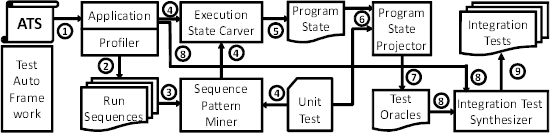
\includegraphics{Workflow}
\caption{The architecture and workflow of ASSIST.}
\label{workflow}
\end{figure}

 
\begin{enumerate}
\item The Application Test Suite(ATS) comprises of AUT, unit and acceptance tests and input data for these tests.
\item AUT is run using with a profiler which collects \textit{run sequences} (execution traces) which contain method names and class names.
\item Run Sequences are analysed by Sequence Pattern Miner that mines patterns from the various runs.\label{3}
\item A subset of the most informative run sequences are submitted to the State Carver.\label{4}
\item State Carver extracts the state of heap memory in the execution of the AUT before the extracted patterns are run.
\item Using unit tests and state of the system Program State Projector determines test oracles.
\item These oracles and source code of AUT are used by Integration Test Synthesizer. 
\item Integration tests are outputted.
\end{enumerate} 
% Chapter 3

\chapter{Project Requirements} % Main chapter title

\label{Chapter3} % For referencing the chapter elsewhere, use \ref{Chapter3} 

\lhead{Chapter 3. \emph{Requirements}} % This is for the header on each page - perhaps a shortened title

%----------------------------------------------------------------------------------------

\section{Requirements}
As seen in Chapter \ref{Chapter2} - \ref{Organization}, this project deals with steps \ref{3} and \ref{4}. We can assume them to be the main requirements. I will re-iterate them as follows:

\begin{itemize}
\item Run Sequences are analysed by Sequence Pattern Miner that mines patterns from the various runs.

\item A subset of the most informative run sequences are submitted to the State Carver.
\end{itemize}

We will see them on a higher level:

\subsection{Finding Frequent Sequences}
\subsubsection{Get the files of Run Sequences(in the format of JSON files)}
The project receives JSON (a data fromat explained in Chapter-\ref{Chapter4}) files and this becomes the primary input to the project . This file has all the Run Sequences with various information like a unique id, method name , class name, etc. A format is also provided and explained in detail in the Chapter-\ref{Chapter4}. We need to parse and read the files for further use.
\subsubsection{BIDE Input generation}
To find the frequent sequences we use a sequential pattern miner BIDE developed and maintained by University of Illinois at Urbana Champagne.
For that we make an input file for the Sequential Pattern Miner(BIDE\cite{Wang:2004:BEM:977401.978142} explained in Chapter- \ref{Chapter4}). The input file requires a special format as a text file and also some statistics about the data in a spec file, like longest sequence, average sequence etc. which needs to be generated from the run sequences and fed to BIDE.


\subsection{Mine Informative Sequences}

\subsubsection{Find all possible valid sequences}
 Use BIDE output file(containing frequent sequences) to mine the Run Sequences and find all the \textit{occurences} of the frequent sequences from the input JSON file. This seems to be a straightforward requirement but it requires careful consideration of many corner cases and with increasing sequence length the problem takes exponential time to solve. We have devised an algorithm to take care of the problem.
 For eg. \{1 2 4 10\} is a frequent sequence and to find it out in a following run sequence \{1 2 4 10 12 3 5 7 4 2 7 4 8 10\} is a daunting task as we need to find all the possible occurences of the frequent sequence not considering its place in the run sequence meaning \{1 2 4 10\} at places \textless1 2 3 4\textgreater and \textless1 10 12 14\textgreater both are of importance as they are different in order of occuring in a particular run sequence and they both need to be tested as their states are most probably different to each other and thus will provide us with different information when tested.
\subsubsection{Pruning}
Applying the heuristic to get the \textit{shortest distance frequent sequences} or \textit{ranked shortest distance frequent sequences}. This prunes the solution space by a big factor and thus simplifies further situations.
Shortest distance is as in the above example \{1 2 4 10\} at places \{1 2 3 4\} which is the shortest distance apart from another.
Ranked shortest distance is the first \textit{n} shortest sequences.
\subsubsection{Output File}
Returning the subset of Run Sequences back in a JSON file.




% Chapter 4

\chapter{Tools and Utilities} % Main chapter title

\label{Chapter4} % For referencing the chapter elsewhere, use \ref{Chapter4} 

\lhead{Chapter 4. \emph{Tools and Utilities}} % This is for the header on each page - perhaps a shortened title

%----------------------------------------------------------------------------------------

\section{JSON(JavaScript Object Notation)}
\subsection{Language Overview}
JSON \cite{JSON-standard} (JavaScript Object Notation) is a lightweight data-interchange format.It is easy for humans to read and write. It is easy for machines to parse and generate. It is based on a subset of the JavaScript Programming Language.JSON is a text format that is completely language independent but uses conventions that are familiar to programmers of the C-family of languages, including C, C++, C\#, Java, JavaScript, Perl, Python, and many others. These properties make JSON an ideal data-interchange language.

JSON has only two structures:
\begin{enumerate}
\item A collection of name/value pairs. In various languages, this is realized as an object, record, struct, dictionary, hash table, keyed list, or associative array.
\item An ordered list of values. In most languages, this is realized as an array, vector, list, or sequence.
\end{enumerate}
These are universal data structures. Virtually all modern programming languages support them in one form or another. It makes sense that a data format that is interchangeable with programming languages also be based on these structures.

In JSON, they take on these forms:
\begin{enumerate}
\item An object is an unordered set of name/value pairs. An object begins with \{ (left brace) and ends with \} (right brace). Each name is followed by : (colon) and the name/value pairs are separated by , (comma).
\item An array is an ordered collection of values. An array begins with [ (left bracket) and ends with ] (right bracket). Values are separated by , (comma).
\item A value can be a string in double quotes, or a number, or true or false or null, or an object or an array. These structures can be nested.
\item A string is a sequence of zero or more Unicode characters, wrapped in double quotes, using backslash escapes. A character is represented as a single character string. A string is very much like a C or Java string.
\item A number is very much like a C or Java number, except that the octal and hexadecimal formats are not used.
\item Whitespace can be inserted between any pair of tokens. Excepting a few encoding details, that completely describes the language.
\end{enumerate}

\subsection{json-simple(Parser API)}
JSON.simple\cite{JSON-simple} is a simple Java toolkit for JSON by google.
It has following features:
\begin{itemize}
\item Full compliance with JSON specification (RFC4627) and reliable (see compliance testing).
\item Provides multiple functionalities such as encode, decode/parse and escape JSON text while keeping the library lightweight.
\item Flexible, simple and easy to use by reusing Map and List interfaces.
\item Supports streaming output of JSON text.
\item Stoppable SAX-like interface for streaming input of JSON text (learn more).
\item Heap based parser.
\item High performance (see performance testing).
\item No dependency on external libraries.
\item Both of the source code and the binary are JDK1.2 compatible.
\end{itemize}

\section{Formats}
\subsection{Input File Format}
There will be two files coming in to the project, the sequence file stating the run sequences of the system. Each run system is described by the function calls called in order for that particular run. They are denoted by number here which is mapped in another file with the other details like the method name and class name. It is possible that the same method be called multiple amounts of time in a single run and thus a counter number is associated to uniquely identify the method at that position.

\begin{enumerate}
\item Method Trace:

[\{"counter": 0, "class-name": "com.ser.instrument.artifacts.InstrumentClass1", "method-name": "int methodWithPrimitiveInt(int)", "level": 28\},\\
 \{"counter": 1, "class-name": "com.ser.instrument.artifacts.InstrumentClass1", "method-name": "int methodWithPrimitiveInt(int)", "level": 29\}\\
]

\item Sequence Map File:

[\{"sequence-no":1, "counters" : [ 1,2, 3, 4, 5, 6, 7, 8, 9, 10]\},\\
 \{"sequence-no": 2, "counters" : [ 5, 7, 8, 10, 13, 15]\}\\
]

\end{enumerate}

\subsection{Output File Format}
There will be one output file generated which will have the frequent sequences for each run provided in the input file.
This basically is an array for each frequent sequence(here called method-sequence). With each frequent sequence we attach the counters at each run sequence.

Output:

[ \{"method-sequence" : [ 1, 3, 4 ],\\
\tab   "occurences" :\\
\tab\tab             { [\{ "sequence-no" : 1,\\
\tab\tab               "counters" : [ 100, 102, 103] \},\\
\tab\tab              \{ "sequence-no":  2,\\
\tab\tab                "counters" : [ 100, 102, 105] \},\\
\tab\tab                \{ "sequence-no" : 3,\\
\tab\tab                  "counters" : [ 500, 501, 510] \}\\
\tab\tab                  ]}\},\\
\\
  \{"method-sequence" : [ 8 ,9, 10 ],\\
\tab   "occurences" :\\
\tab\tab             { [\{ "sequence-no" : 8,\\
\tab\tab                "counters" : [ 100, 102, 103] \},\\
\tab\tab                \{ "sequence-no":  9,\\
\tab\tab                "counters" : [ 100, 102, 105] \},\\
\tab\tab                \{ "sequence-no" : 10,\\
\tab\tab                  "counters" : [ 500, 501, 510] \}\\
\tab\tab                  ]}\}\\
]

%----------------------------------------------------------------------------------------
\section{Maven}
\subsection{Overview}
Maven\cite{Maven} is a build tool made available by Apache. There are various uses of this tool as described below:

\begin{itemize}
\item Making the build process easy.
\item Providing a uniform build system.
\item Providing quality project information.
\item Providing guidelines for best practices development.
\item Allowing transparent migration to new features.
\end{itemize}

\subsection{Project Hierarchy}
Maven provides a well organized heirarchy for the project separating test and source folders in test and main folders.
The snapshot of the project heirarchy is shown in Fig.\ref{heirarchy}.

\begin{figure}[h]
\centering
 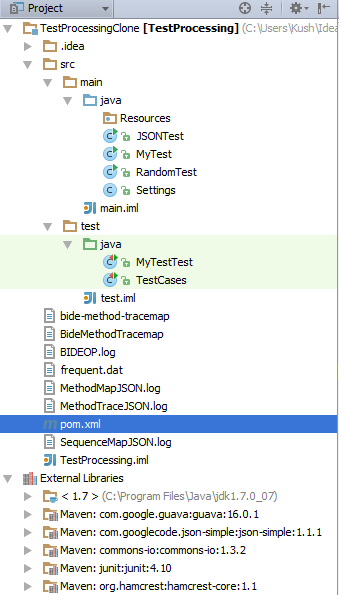
\includegraphics{maven_heirarchy}
\caption{Project Heirarchy.}
\label{heirarchy}
\end{figure}

\subsection{Project Object Model}
A Project Object Model or POM\cite{pom} is the fundamental unit of work in Maven. It is an XML file that contains information about the project and configuration details used by Maven to build the project. It contains default values for most projects. Examples for this is the build directory, which is target; the source directory, which is src/main/java; the test source directory, which is src/main/test; and so on.\\

The main use of the file is to include jar files of external resources like json parser, junit, etc. The build tool fetches the jars from the internet and is thus useful while collaborating as only pom.xml can be shared instead of the physical jar themselves.\\


Following Fig.\ref{pom} is the pom.xml for the project:
\begin{figure}[h]
\centering
 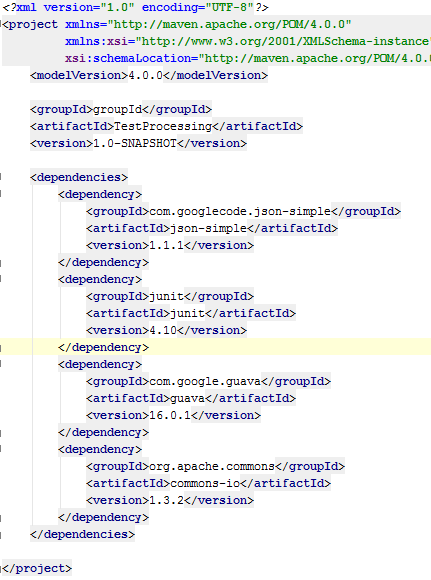
\includegraphics{maven_pom}
\caption{pom.xml.}
\label{pom}
\end{figure}

\section{BIDE (BI-Directional Extension based frequent closed sequence mining)}
\subsection{Overview}
The goal of using this tool is to mine frequent patterns of method invocations invoked in execution traces that were collected by the profiler from the AUT with acceptance and get models of interactions among different components.

Frequent patterns are sequences occuring in the dataset more than a predefined and user defined threshold value\cite{Han:2007:FPM:1275092.1275097}.

For example, a person visits a mall every week and buys some items. He will have a list of items that he bought, suppose each as a row in the dataset. If for assumption, milk and bread appear more than the threshold value, in the rows, they are called as Frequent Sequential Pattern.

 \{1 2 4 10\} is a frequent sequence in a following run sequence \{1 2 4 10 12 3 5 7 4 2 7 4 8 10\} 
 This sequence is closed and maximal because they are the biggest sequences that are not present in larger and equally or higher frequent sequences.
 
 Thus, we need a miner developed by academicians from University of Illinois at Urbana- Champagne \cite{Wang:2004:BEM:977401.978142}
 It is a very easy to use executable which can be used by accessing the operating system process for running it.
 
 Let us go through the details of using BIDE:
 
\subsubsection{Input parameters}
\tab1st argument: The specification file of the dataset\\
\tab2nd argument: Relative support in decimal\\
Usage example: bide $bide_input$.spec 0.0002\\
Where bide is the executable file name, $bide_input$.spec is the specification file of the sequence dataset being mined, 0.0002 is the relative support.
As to the dataset file format, see section 4.4.1.4.

\subsubsection{Output}
The discovered frequent sequences are printed into a file called “frequent.dat”.\\
Each line in the result file, “frequent.dat”, contains a frequent sequence in the form:\\
event1 event2 … eventn : absolute support\\
Here is an example:\\
6 24 748 : 66\\


\subsubsection{Specification file format}
The first line is the dataset file name.\\
The second line is the number of unique items.\\ 
The third line is the number of sequences.\\ 
The fourth line is the maximal length of a sequence.\\
The fifth line is the average length of a sequence.

\subsubsection{Dataset file format}
Usually a sequence database consists of a series of sequences (strictly speaking, here a sequence is a string in the current implementation). Each line represents a sequence and ends with -1, and the entire dataset ends with -2.\\
Here is a sample sequence:\\
In our case each number is an item in run sequence more precisely a function invocation.\\
And each line represents a different run sequence.\\
For eg.\\
1 4 35 90 -1\\
1 2 3 54 77 -1\\
-2

\subsection{Other Tools}
\begin{enumerate}
\item Java Standard Edition Development Kit 7 for coding. 
\item IntelliJ (Intgrated Development Environment).
\item HP-ENVY 4 Laptop for all the experiments.
\item GitHub online repository for collaboration.
\item Tortoise SVN for version control.
\end{enumerate}


 
% Chapter 5

\chapter{Implementation} % Main chapter title

\label{Chapter5} % For referencing the chapter elsewhere, use \ref{Chapter5} 

\lhead{Chapter 5. \emph{Algorithms}} % This is for the header on each page - perhaps a shortened title

%----------------------------------------------------------------------------------------

\section{Correct Sequences}
Suppose the following are a run sequence and a frequent sequence.
We need to find out if the frequent sequence is present in a run sequence. But how do we decide of all the combinations possible which ones to select?

\subsection{Run Sequence}
Run Sequences are provided as input in a JSON file. They denote the order of the  method invocations of the acceptance test.\\
\begin{tabular}{l|llllllllllllllll}
run sequence& 1 &4 &5 &4 &36 &84 &1 &3 &4 &5 &8 &17 &99 &8 &32 &9\\
\hline
 counters&0 &1 &2 &3 &4  &5  &6  &7  &8  &9 &10 &11 &12 &13 &14 &15 \\
\end{tabular}

\subsection{Frequent Sequence}
Frequent Sequence is one of the many output sequences that BIDE provide in frequent.dat file.
It is closed and maximal
Suppose one of the frequent sequence is 1 4 5

\subsection{Analysis}
So let's see which of the few possible sequences are correct or useful for us.\\
As there can be repetetive functions for the same run sequence, we will uniquely identify the method with respect to the counter number.

\checkmark\tab 0 1 2\\
\tab This is a straightforward consecutive sequence and is valid.

\checkmark \tab0 3 9\\
\tab This is also a valid sequence as 1 4 5 appear in order though they are not consecutive.

{\large{X}}\tab 6 3 9\\
\tab This will not be considered valid because though the counters suggest 1 4 5 but they are not in order and with respect to integration testing run sequences are ordered so in other words we donot have the state of functions in that order and thus we are not interested in these types of sequences as they do not occur.

\section{Block Structure}
The Fig.\ref{algo} explains the basic blocks of the project.\\
They consist of various sub functions and/or helping functions that we will see in the detailed explanation.

\begin{figure}[h]
\centering
 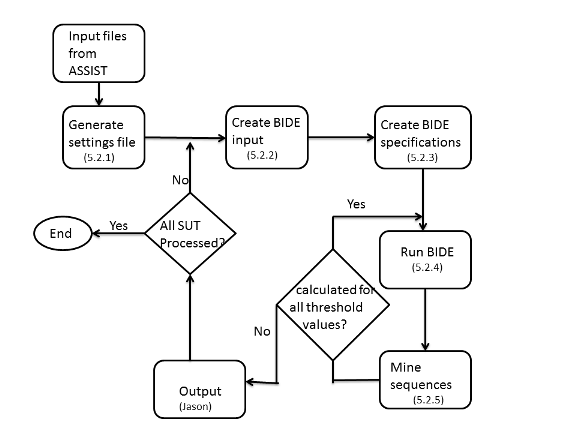
\includegraphics{algo}
\caption{Project Implementation.}
\label{algo}
\end{figure}

\subsection{Generate Settings File}
Before starting the program one needs to set the values of Settings.java file.\\
This is a static class which holds various values which are user inputs and which remain constant throughout the program.\\
They are:
\begin{itemize}
\item basePath : The folder where all the SUT folders reside
\item subjectAppName : The name of the SUT (to be appended to basePath)
\item thresholdValues : The array which stores all the threshold values for BIDE for which the SUT will be tested and results will be stored under the folder basePath/subjectAppName/thresholdValue.
\item methodMapFile : File name format for the input JSON file which maps each method with its name and class name to a unique number
\item sequenceMapFile : File name format for the Run Sequences in JSON file.
\end{itemize}
\tab and similar BIDE related data \dots

\subsection{Create BIDE Input}
This module takes care of converting the Run Sequences in input files from the JSON format to the textual-dataset (format required by the BIDE), explained in the Tools Section.\\
For each Run Sequence the data is extracted from JSON packets and stored in an BIDE input file.

\subsection{Create BIDE Specification}
While parsing the run sequences, ststistics required by the specification file format of BIDE are calculated.
They are:
\begin{itemize}
\item Number of Unique Items(Total number of methods, obtained from methodMap)
\item Number of Sequences(Total number of Run Sequences in input file)
\item Maximum length of sequences(Keeping a track while parsing from JSON)
\item Average length of sequence(Keeping a track while parsing)
\end{itemize}

\subsection{Run BIDE}
This module is called for each value of threshold mentioned in the Settings file.\\
An Operating System Process is borrowed and the BIDE executable is run on a Runtime Data Structure each time the module is called. There are two types of executables, one is with output on console and one is without output. The one with output can be used for logging purposes.

\subsection{Mine Sequences}
This module is the heart of the project. Most of the computative things happen in this module. There are various helper and subfunctions in this module. We will discuss them in detail in the following subsections.

\emph{Global Parameters for the module} : \{JSONObject, JSONArray, iterator, JSONParser\}

Let us see a combined pseudocde for an overview:
\subsubsection{getOccurence()}
\tab\emph{parameters} : Frequent Sequence\\
\tab\emph{return value} : All Subsequences from all the Run Sequences\\
\tab\emph{body} : Iterates over all Run Sequences and calls a helper function getSubSequences()

\subsubsection{getSubSequence()}
\tab\emph{parameters} : Frequent Sequence, Run Sequence, Counters of Run Sequence\\
\tab\emph{return value} : All the Subsequences of a particular Run Sequence\\
\tab\emph{body} : Calls getIndividualSet()\\
\tab\tab\tab 		        do\{\\
\tab\tab\tab\tab				add another item and create all possible combinations\\
\tab\tab\tab\tab				check if combination is a correct one\\
\tab\tab\tab\tab				reject the incorrect combination\\
\tab\tab\tab			\}\\
\tab\tab\tab			while(all items of frequent set covered)\\
This solution is inspired from the classic computer NP-Hard problem of Longest Common Subsequence\cite{lcs}.

			
\subsubsection{getIndividualSet()}
\tab\emph{parameters} : Frequent Sequence, Run Sequence, Counters of Run Sequence\\
\tab\emph{return value} : Sets, for each item in the frequent set, consisting of all the occurences in run sequence\\
\tab\emph{body} : for(each item in frequent set)\{\\
\tab\tab\tab 			for(each item in Run Sequence)\{\\
\tab\tab\tab\tab			if(items match)\{\\
\tab\tab\tab\tab\tab			add counter in the return list\\
\tab\tab\tab\tab 			\}\\
\tab\tab\tab 			\}\\
\tab\tab 		\}\\
				 
% Chapter 6

\chapter{Conclusion} % Main chapter title

\label{Chapter6} % For referencing the chapter elsewhere, use \ref{Chapter6} 

\lhead{Chapter 6. \emph{Conclusion}} % This is for the header on each page - perhaps a shortened title

%----------------------------------------------------------------------------------------

\section{Future Work}
There are several shortcomings to the present version of the project. Following are the enhancements that can be worked upon:

\begin{itemize}
\item Newer heuristics similar to shortest distance can be devised to further help develop better integration tests.
\item Automatic heuristic development can be thought of on the basis of interactions within the AUT.
\item Threshold for a particular AUT varies on the basis of the spread of the Run Sequences. Ways can be devised to intelligently approximate the values to be tested.
\end{itemize}

\section{Conclusion}

In Conclusion MINUSA helps ASSIST in mining useful sequences and pruning less useful sequences from a very big corpus generated. Although the task is resource and time intensive, efficient heuristics can be applied and the aim can be achieved in an acceptable time frame. Results of an application dealing in nanoscience are shown in the Appendix\ref{AppendixA} along with the code files.
 
%% Chapter 2

\chapter{Chapter Title Here} % Main chapter title

\label{Chapter4} % For referencing the chapter elsewhere, use \ref{Chapter1} 

\lhead{Chapter 2. \emph{Chapter Title Here}} % This is for the header on each page - perhaps a shortened title

%----------------------------------------------------------------------------------------

\section{Welcome and Thank You}
Welcome to this \LaTeX{} Thesis Template, a beautiful and easy to use template for writing a thesis using the \LaTeX{} typesetting system.

If you are writing a thesis (or will be in the future) and its subject is technical or mathematical (though it doesn't have to be), then creating it in \LaTeX{} is highly recommended as a way to make sure you can just get down to the essential writing without having to worry over formatting or wasting time arguing with your word processor.

\LaTeX{} is easily able to professionally typeset documents that run to hundreds or thousands of pages long. With simple mark-up commands, it automatically sets out the table of contents, margins, page headers and footers and keeps the formatting consistent and beautiful. One of its main strengths is the way it can easily typeset mathematics, even \emph{heavy} mathematics. Even if those equations are the most horribly twisted and most difficult mathematical problems that can only be solved on a super-computer, you can at least count on \LaTeX{} to make them look stunning.

%----------------------------------------------------------------------------------------

\section{Learning \LaTeX{}}

\LaTeX{} is not a WYSIWYG (What You See is What You Get) program, unlike word processors such as Microsoft Word or Apple's Pages. Instead, a document written for \LaTeX{} is actually a simple, plain text file that contains \emph{no formatting}. You tell \LaTeX{} how you want the formatting in the finished document by writing in simple commands amongst the text, for example, if I want to use \textit{italic text for emphasis}, I write the `$\backslash$\texttt{textit}\{\}' command and put the text I want in italics in between the curly braces. This means that \LaTeX{} is a ``mark-up'' language, very much like HTML.

\subsection{A (not so short) Introduction to \LaTeX{}}

If you are new to \LaTeX{}, there is a very good eBook -- freely available online as a PDF file -- called, ``The Not So Short Introduction to \LaTeX{}''. The book's title is typically shortened to just ``lshort''. You can download the latest version (as it is occasionally updated) from here:\\
\href{http://www.ctan.org/tex-archive/info/lshort/english/lshort.pdf}{\texttt{http://www.ctan.org/tex-archive/info/lshort/english/lshort.pdf}}

It is also available in several other languages. Find yours from the list on this page:\\
\href{http://www.ctan.org/tex-archive/info/lshort/}{\texttt{http://www.ctan.org/tex-archive/info/lshort/}}

It is recommended to take a little time out to learn how to use \LaTeX{} by creating several, small `test' documents. Making the effort now means you're not stuck learning the system when what you \emph{really} need to be doing is writing your thesis.

\subsection{A Short Math Guide for \LaTeX{}}

If you are writing a technical or mathematical thesis, then you may want to read the document by the AMS (American Mathematical Society) called, ``A Short Math Guide for \LaTeX{}''. It can be found online here:\\
\href{http://www.ams.org/tex/amslatex.html}{\texttt{http://www.ams.org/tex/amslatex.html}}\\
under the ``Additional Documentation'' section towards the bottom of the page.

\subsection{Common \LaTeX{} Math Symbols}
There are a multitude of mathematical symbols available for \LaTeX{} and it would take a great effort to learn the commands for them all. The most common ones you are likely to use are shown on this page:\\
\href{http://www.sunilpatel.co.uk/latexsymbols.html}{\texttt{http://www.sunilpatel.co.uk/latexsymbols.html}}

You can use this page as a reference or crib sheet, the symbols are rendered as large, high quality images so you can quickly find the \LaTeX{} command for the symbol you need.

\subsection{\LaTeX{} on a Mac}
 
The \LaTeX{} package is available for many systems including Windows, Linux and Mac OS X. The package for OS X is called MacTeX and it contains all the applications you need -- bundled together and pre-customised -- for a fully working \LaTeX{} environment and workflow.
 
MacTeX includes a dedicated \LaTeX{} IDE (Integrated Development Environment) called ``TeXShop'' for writing your `\texttt{.tex}' files and ``BibDesk'': a program to manage your references and create your bibliography section just as easily as managing songs and creating playlists in iTunes.

%----------------------------------------------------------------------------------------

\section{Getting Started with this Template}

If you are familiar with \LaTeX{}, then you can familiarise yourself with the contents of the Zip file and the directory structure and then place your own information into the `\texttt{Thesis.cls}' file. Section \ref{FillingFile} on page \pageref{FillingFile} tells you how to do this. Make sure you read section \ref{ThesisConventions} about thesis conventions to get the most out of this template and then get started with the `\texttt{Thesis.tex}' file straightaway.

If you are new to \LaTeX{} it is recommended that you carry on reading through the rest of the information in this document.

\subsection{About this Template}

This \LaTeX{} Thesis Template is originally based and created around a \LaTeX{} style file created by Steve R.\ Gunn from the University of Southampton (UK), department of Electronics and Computer Science. You can find his original thesis style file at his site, here:\\
\href{http://www.ecs.soton.ac.uk/~srg/softwaretools/document/templates/}{\texttt{http://www.ecs.soton.ac.uk/$\sim$srg/softwaretools/document/templates/}}

My thesis originally used the `\texttt{ecsthesis.cls}' from his list of styles. However, I knew \LaTeX{} could still format better. To get the look I wanted, I modified his style and also created a skeleton framework and folder structure to place the thesis files in.

This Thesis Template consists of that modified style, the framework and the folder structure. All the work that has gone into the preparation and groundwork means that all you have to bother about is the writing.

Before you begin using this template you should ensure that its style complies with the thesis style guidelines imposed by your institution. In most cases this template style and layout will be suitable. If it is not, it may only require a small change to bring the template in line with your institution's recommendations.

%----------------------------------------------------------------------------------------

\section{What this Template Includes}

\subsection{Folders}

This template comes as a single Zip file that expands out to many files and folders. The folder names are mostly self-explanatory:

\textbf{Appendices} -- this is the folder where you put the appendices. Each appendix should go into its own separate `\texttt{.tex}' file. A template is included in the directory.

\textbf{Chapters} -- this is the folder where you put the thesis chapters. A thesis usually has about seven chapters, though there is no hard rule on this. Each chapter should go in its own separate `\texttt{.tex}' file and they usually are split as:
\begin{itemize}
\item Chapter 1: Introduction to the thesis topic
\item Chapter 2: Background information and theory
\item Chapter 3: (Laboratory) experimental setup
\item Chapter 4: Details of experiment 1
\item Chapter 5: Details of experiment 2
\item Chapter 6: Discussion of the experimental results
\item Chapter 7: Conclusion and future directions
\end{itemize}
This chapter layout is specialised for the experimental sciences.

\textbf{Figures} -- this folder contains all figures for the thesis. These are the final images that will go into the thesis document.

\textbf{Primitives} -- this is the folder that contains scraps, particularly because one final image in the `Figures' folder may be made from many separate images and photos, these source images go here. This keeps the intermediate files separate from the final thesis figures.

\subsection{Files}

Included are also several files, most of them are plain text and you can see their contents in a text editor. Luckily, many of them are auxiliary files created by \LaTeX{} or BibTeX and which you don't need to bother about:

\textbf{Bibliography.bib} -- this is an important file that contains all the bibliographic information and references that you will be citing in the thesis for use with BibTeX. You can write it manually, but there are reference manager programs available that will create and manage it for you. Bibliographies in \LaTeX{} are a large subject and you may need to read about BibTeX before starting with this.

\textbf{Thesis.cls} -- this is an important file. It is the style file that tells \LaTeX{} how to format the thesis. You will also need to open this file in a text editor and fill in your own information (such as name, department, institution). Luckily, this is not too difficult and is explained in section \ref{FillingFile} on page \pageref{FillingFile}.

\textbf{Thesis.pdf} -- this is your beautifully typeset thesis (in the PDF file format) created by \LaTeX{}.

\textbf{Thesis.tex} -- this is an important file. This is the file that you tell \LaTeX{} to compile to produce your thesis as a PDF file. It contains the framework and constructs that tell \LaTeX{} how to layout the thesis. It is heavily commented so you can read exactly what each line of code does and why it is there. After you put your own information into the `\texttt{Thesis.cls}' file, go to this file and begin filling it in -- you have now started your thesis!

\textbf{vector.sty} -- this is a \LaTeX{} package, it tells \LaTeX{} how to typeset mathematical vectors. Using this package is very easy and you can read the documentation on the site (you just need to look at the `\texttt{vector.pdf}' file):\\
\href{http://www.ctan.org/tex-archive/macros/latex/contrib/vector/}{\texttt{http://www.ctan.org/tex-archive/macros/latex/contrib/vector/}}

\textbf{lstpatch.sty} -- this is a \LaTeX{} package required by this LaTeX template and is included as not all \TeX{} distributions have it installed by default. You do not need to modify this file.

Files that are \emph{not} included, but are created by \LaTeX{} as auxiliary files include:

\textbf{Thesis.aux} -- this is an auxiliary file generated by \LaTeX{}, if it is deleted \LaTeX{} simply regenerates it when you run the main `\texttt{.tex}' file.

\textbf{Thesis.bbl} -- this is an auxiliary file generated by BibTeX, if it is deleted, BibTeX simply regenerates it when you run the main tex file. Whereas the `\texttt{.bib}' file contains all the references you have, this `\texttt{.bbl}' file contains the references you have actually cited in the thesis and is used to build the bibliography section of the thesis.

\textbf{Thesis.blg} -- this is an auxiliary file generated by BibTeX, if it is deleted BibTeX simply regenerates it when you run the main `\texttt{.tex}' file.

\textbf{Thesis.lof} -- this is an auxiliary file generated by \LaTeX{}, if it is deleted \LaTeX{} simply regenerates it when you run the main `\texttt{.tex}' file. It tells \LaTeX{} how to build the `List of Figures' section.

\textbf{Thesis.log} -- this is an auxiliary file generated by \LaTeX{}, if it is deleted \LaTeX{} simply regenerates it when you run the main `\texttt{.tex}' file. It contains messages from \LaTeX{}, if you receive errors and warnings from \LaTeX{}, they will be in this `\texttt{.log}' file.

\textbf{Thesis.lot} -- this is an auxiliary file generated by \LaTeX{}, if it is deleted \LaTeX{} simply regenerates it when you run the main `\texttt{.tex}' file. It tells \LaTeX{} how to build the `List of Tables' section.

\textbf{Thesis.out} -- this is an auxiliary file generated by \LaTeX{}, if it is deleted \LaTeX{} simply regenerates it when you run the main `\texttt{.tex}' file.


So from this long list, only the files with the `\texttt{.sty}', `\texttt{.bib}', `\texttt{.cls}' and `\texttt{.tex}' extensions are the most important ones. The other auxiliary files can be ignored or deleted as \LaTeX{} and BibTeX will regenerate them.

%----------------------------------------------------------------------------------------

\section{Filling in the `\texttt{Thesis.cls}' File}\label{FillingFile}

You will need to personalise the thesis template and make it your own by filling in your own information. This is done by editing the `\texttt{Thesis.cls}' file in a text editor.

Open the file and scroll down, past all the `$\backslash$\texttt{newcommand}\ldots' items until you see the entries for `\texttt{University Name}', `\texttt{Department Name}', etc\ldots.

Fill out the information about your group and institution and ensure you keep to block capitals where it asks you to. You can also insert web links, if you do, make sure you use the full URL, including the `\texttt{http://}' for this.

The last item you should need to fill in is the Faculty Name (in block capitals). When you have done this, save the file and recompile `\texttt{Thesis.tex}'. All the information you filled in should now be in the PDF, complete with web links. You can now begin your thesis proper!

%----------------------------------------------------------------------------------------

\section{The `\texttt{Thesis.tex}' File Explained}

The \texttt{Thesis.tex} file contains the structure of the thesis. There are plenty of written comments that explain what pages, sections and formatting the \LaTeX{} code is creating. Initially there seems to be a lot of \LaTeX{} code, but this is all formatting, and it has all been taken care of so you don't have to do it.

Begin by checking that your information on the title page is correct. For the thesis declaration, your institution may insist on something different than the text given. If this is the case, just replace what you see with what is required.

Then comes a page which contains a funny quote. You can put your own, or quote your favourite scientist, author, person, etc\ldots Make sure to put the name of the person who you took the quote from.

Next comes the acknowledgements. On this page, write about all the people who you wish to thank (not forgetting parents, partners and your advisor/supervisor).

The contents pages, list of figures and tables are all taken care of for you and do not need to be manually created or edited. The next set of pages are optional and can be deleted since they are for a more technical thesis: insert a list of abbreviations you have used in the thesis, then a list of the physical constants and numbers you refer to and finally, a list of mathematical symbols used in any formulae. Making the effort to fill these tables means the reader has a one-stop place to refer to instead of searching the internet and references to try and find out what you meant by certain abbreviations or symbols.

The list of symbols is split into the Roman and Greek alphabets. Whereas the abbreviations and symbols ought to be listed in alphabetical order (and this is \emph{not} done automatically for you) the list of physical constants should be grouped into similar themes.

The next page contains a one line dedication. Who will you dedicate your thesis to?

Finally, there is the section where the chapters are included. Uncomment the lines (delete the `\texttt{\%}' character) as you write the chapters. Each chapter should be written in its own file and put into the `Chapters' folder and named `\texttt{Chapter2}', `\texttt{Chapter2}, etc\ldots Similarly for the appendices, uncomment the lines as you need them. Each appendix should go into its own file and placed in the `Appendices' folder.

After the preamble, chapters and appendices finally comes the bibliography. The bibliography style (called `\texttt{unsrtnat}') is used for the bibliography and is a fully featured style that will even include links to where the referenced paper can be found online. Do not under estimate how grateful you reader will be to find that a reference to a paper is just a click away. Of course, this relies on you putting the URL information into the BibTeX file in the first place.

%----------------------------------------------------------------------------------------

\section{Thesis Features and Conventions}\label{ThesisConventions}

To get the best out of this template, there are a few conventions that you may want to follow.

One of the most important (and most difficult) things to keep track of in such a long document as a thesis is consistency. Using certain conventions and ways of doing things (such as using a Todo list) makes the job easier. Of course, all of these are optional and you can adopt your own method.

\subsection{Printing Format}

This thesis template is designed for single sided printing as most theses are printed and bound this way. This means that the left margin is always wider than the right (for binding). Four out of five people will now judge the margins by eye and think, ``I never 
noticed that before.''.

The headers for the pages contain the page number on the right side (so it is easy to flick through to the page you want) and the chapter name on the left side.

The text is set to 1 point and a line spacing of 1.3. Generally, it is much more readable to have a smaller text size and wider gap between the lines than it is to have a larger text size and smaller gap. Again, you can tune the text size and spacing should you want or need to. The text size can be set in the options for the `$\backslash$\texttt{documentclass}' command at the top of the `\texttt{Thesis.tex}' file and the spacing can be changed by setting a different value in the `$\backslash$\texttt{setstretch}' commands (scattered throughout the `\texttt{Thesis.tex}' file).

\subsection{Using US Letter Paper}

The paper size used in the template is A4, which is a common -- if not standard -- size in Europe. If you are using this thesis template elsewhere and particularly in the United States, then you may have to change the A4 paper size to the US Letter size. Unfortunately, this is not as simple as replacing instances of `\texttt{a4paper}' with `\texttt{letterpaper}'.

This is because the final PDF file is created directly from the \LaTeX{} source using a program called `\texttt{pdfTeX}' and in certain conditions, paper size commands are ignored and all documents are created with the paper size set to the size stated in the configuration file for pdfTeX (called `\texttt{pdftex.cfg}').

What needs to be done is to change the paper size in the configuration file for \texttt{pdfTeX} to reflect the letter size. There is an excellent tutorial on how to do this here: \\
\href{http://www.physics.wm.edu/~norman/latexhints/pdf_papersize.html}{\texttt{http://www.physics.wm.edu/$\sim$norman/latexhints/pdf\_papersize.html}}

It may be sufficient just to replace the dimensions of the A4 paper size with the US Letter size in the \texttt{pdftex.cfg} file. Due to the differences in the paper size, the resulting margins may be different to what you like or require (as it is common for Institutions to dictate certain margin sizes). If this is the case, then the margin sizes can be tweaked by opening up the \texttt{Thesis.cls} file and searching for the line beginning with, `$\backslash$\texttt{setmarginsrb}' (not very far down from the top), there you will see the margins specified. Simply change those values to what you need (or what looks good) and save. Now your document should be set up for US Letter paper size with suitable margins.

\subsection{References}

The `\texttt{natbib}' package is used to format the bibliography and inserts references such as this one \citep{Reference3}. The options used in the `\texttt{Thesis.tex}' file mean that the references are listed in numerical order as they appear in the text. Multiple references are rearranged in numerical order (e.g. \citep{Reference2, Reference1}) and multiple, sequential references become reformatted to a reference range (e.g. \citep{Reference2, Reference1, Reference3}). This is done automatically for you. To see how you use references, have a look at the `\texttt{Chapter2.tex}' source file. Many reference managers allow you to simply drag the reference into the document as you type.

Scientific references should come \emph{before} the punctuation mark if there is one (such as a comma or period). The same goes for footnotes\footnote{Such as this footnote, here down at the bottom of the page.}. You can change this but the most important thing is to keep the convention consistent throughout the thesis. Footnotes themselves should be full, descriptive sentences (beginning with a capital letter and ending with a full stop).

To see how \LaTeX{} typesets the bibliography, have a look at the very end of this document (or just click on the reference number links).

\subsection{Figures}

There will hopefully be many figures in your thesis (that should be placed in the `Figures' folder). The way to insert figures into your thesis is to use a code template like this:
\begin{verbatim}
\begin{figure}[htbp]
  \centering
    
\includegraphics{Figures/Electron.pdf}
    \rule{35em}{0.5pt}
  \caption[An Electron]{An electron (artist's impression).}
  \label{fig:Electron}
\end{figure}
\end{verbatim}
Also look in the source file. Putting this code into the source file produces the picture of the electron that you can see in the figure below.

\begin{figure}[htbp]
	\centering
		
\includegraphics{Figures/Electron.pdf}
		\rule{35em}{0.5pt}
	\caption[An Electron]{An electron (artist's impression).}
	\label{fig:Electron}
\end{figure}

Sometimes figures don't always appear where you write them in the source. The placement depends on how much space there is on the page for the figure. Sometimes there is not enough room to fit a figure directly where it should go (in relation to the text) and so \LaTeX{} puts it at the top of the next page. Positioning figures is the job of \LaTeX{} and so you should only worry about making them look good!

Figures usually should have labels just in case you need to refer to them (such as in Figure \ref{fig:Electron}). The `$\backslash$\texttt{caption}' command contains two parts, the first part, inside the square brackets is the title that will appear in the `List of Figures', and so should be short. The second part in the curly brackets should contain the longer and more descriptive caption text.

The `$\backslash$\texttt{rule}' command is optional and simply puts an aesthetic horizontal line below the image. If you do this for one image, do it for all of them.

The \LaTeX{} Thesis Template is able to use figures that are either in the PDF or JPEG file format.

\subsection{Typesetting mathematics}

If your thesis is going to contain heavy mathematical content, be sure that \LaTeX{} will make it look beautiful, even though it won't be able to solve the equations for you.

The ``Not So Short Introduction to \LaTeX{}'' (available \href{http://www.ctan.org/tex-archive/info/lshort/english/lshort.pdf}{here}) should tell you everything you need to know for most cases of typesetting mathematics. If you need more information, a much more thorough mathematical guide is available from the AMS called, ``A Short Math Guide to \LaTeX{}'' and can be downloaded from:\\
\href{ftp://ftp.ams.org/pub/tex/doc/amsmath/short-math-guide.pdf}{\texttt{ftp://ftp.ams.org/pub/tex/doc/amsmath/short-math-guide.pdf}}

There are many different \LaTeX{} symbols to remember, luckily you can find the most common symbols \href{http://www.sunilpatel.co.uk/latexsymbols.html}{here}. You can use the web page as a quick reference or crib sheet and because the symbols are grouped and rendered as high quality images (each with a downloadable PDF), finding the symbol you need is quick and easy.

You can write an equation, which is automatically given an equation number by \LaTeX{} like this:
\begin{verbatim}
\begin{equation}
E = mc^{2}
  \label{eqn:Einstein}
\end{equation}
\end{verbatim}

This will produce Einstein's famous energy-matter equivalence equation:
\begin{equation}
E = mc^{2}
\label{eqn:Einstein}
\end{equation}

All equations you write (which are not in the middle of paragraph text) are automatically given equation numbers by \LaTeX{}. If you don't want a particular equation numbered, just put the command, `$\backslash$\texttt{nonumber}' immediately after the equation.

%----------------------------------------------------------------------------------------

\section{Sectioning and Subsectioning}

You should break your thesis up into nice, bite-sized sections and subsections. \LaTeX{} automatically builds a table of Contents by looking at all the `$\backslash$\texttt{chapter}$\{\}$', `$\backslash$\texttt{section}$\{\}$' and `$\backslash$\texttt{subsection}$\{\}$' commands you write in the source.

The table of Contents should only list the sections to three (3) levels. A `$\backslash$\texttt{chapter}$\{\}$' is level one (1). A `$\backslash$\texttt{section}$\{\}$' is level two (2) and so a `$\backslash$\texttt{subsection}$\{\}$' is level three (3). In your thesis it is likely that you will even use a `$\backslash$\texttt{subsubsection}$\{\}$', which is level four (4). Adding all these will create an unnecessarily cluttered table of Contents and so you should use the `$\backslash$\texttt{subsubsection$^{*}\{\}$}' command instead (note the asterisk). The asterisk ($^{*}$) tells \LaTeX{} to omit listing the subsubsection in the Contents, keeping it clean and tidy.

%----------------------------------------------------------------------------------------

\section{In Closing}

You have reached the end of this mini-guide. You can now rename or overwrite this pdf file and begin writing your own `\texttt{Chapter2.tex}' and the rest of your thesis. The easy work of setting up the structure and framework has been taken care of for you. It's now your job to fill it out!

Good luck and have lots of fun!

\begin{flushright}
Guide written by ---\\
Sunil Patel: \href{http://www.sunilpatel.co.uk}{www.sunilpatel.co.uk}
\end{flushright}
 

%----------------------------------------------------------------------------------------
%	REPORT CONTENT - APPENDICES
%----------------------------------------------------------------------------------------

\addtocontents{toc}{\vspace{2em}} % Add a gap in the Contents, for aesthetics

\appendix % Cue to tell LaTeX that the following 'chapters' are Appendices

% Include the appendices of the report as separate files from the Appendices folder
% Uncomment the lines as you write the Appendices

% Appendix A

\chapter{Results and Code} % Main appendix title

\label{AppendixA} % For referencing this appendix elsewhere, use \ref{AppendixA}

\lhead{Appendix A. \emph{Results and Code}} % This is for the header on each page - perhaps a shortened title

\section{Results}
As seen in the Fig.\ref{shortestsubsequence} method-sequence is the Frequent Sequence and sequence number denotes the Run Sequence and thus for each Frequent Sequence all occurences from all Run Sequence are shown. The list is exhaustive even for the shortest distance hueristic and thus only a snippet is shown.\\
All the results and code are available at the \href{https://github.com/kushshah/TestProcessing}{Online repository}.\\
\begin{figure}[h]
 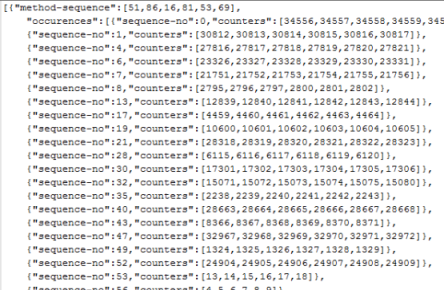
\includegraphics{shortestsubsequence}
\caption{Results of one of the thresholds for Shortest SubSequence.}
\label{shortestsubsequence}
\end{figure}

\section{Settings.java}
\lstset{language=Java, caption=Settings.java, label=DescriptiveLabel,breaklines=true,breakatwhitespace=false,keywordstyle=\color{blue},identifierstyle=\color{black},commentstyle=\color{green}}
\lstinputlisting{Settings.java}

\section{MyTest.java}
\lstset{language=Java, caption=MyTest.java, label=DescriptiveLabel,breaklines=true,breakatwhitespace=false,keywordstyle=\color{blue},identifierstyle=\color{black},commentstyle=\color{green}}
\lstinputlisting{abcd.java}
%\input{Appendices/AppendixB}
%\input{Appendices/AppendixC}

\addtocontents{toc}{\vspace{2em}} % Add a gap in the Contents, for aesthetics

\backmatter

%----------------------------------------------------------------------------------------
%	BIBLIOGRAPHY
%----------------------------------------------------------------------------------------

\label{Bibliography}

\lhead{\emph{Bibliography}} % Change the page header to say "Bibliography"

\bibliographystyle{unsrtnat} % Use the "unsrtnat" BibTeX style for formatting the Bibliography

\bibliography{Bibliography} % The references (bibliography) information are stored in the file named "Bibliography.bib"

\end{document}  